% Created 2022-05-05 Do 10:09
% Intended LaTeX compiler: pdflatex
\documentclass[presentation]{beamer}
\usepackage[utf8]{inputenc}
\usepackage[T1]{fontenc}
\usepackage{graphicx}
\usepackage{grffile}
\usepackage{longtable}
\usepackage{wrapfig}
\usepackage{rotating}
\usepackage[normalem]{ulem}
\usepackage{amsmath}
\usepackage{textcomp}
\usepackage{amssymb}
\usepackage{capt-of}
\usepackage{hyperref}
\usepackage{minted}
\usepackage[utf8]{inputenc}
\usepackage{color}
\usetheme[height=7mm]{Rochester}
\setbeamertemplate{footline}[frame number]
\usecolortheme[accent=red, light]{solarized}
\setbeamercolor{frametitle}{bg=solarizedRebase02,fg=solarizedAccent}
\setbeamercolor{author in head/foot}{bg=solarizedRebase02,fg=solarizedRebase01}
\setbeamercolor{title in head/foot}{bg=solarizedRebase02,fg=solarizedRebase01}
\setbeamercolor{block title}{bg=solarizedRebase0,fg=solarizedRebase02}
\setbeamercolor{block body}{bg=solarizedRebase02,fg=solarizedRebase0}
\setbeamercolor{item}{bg=solarizedRebase02,fg=solarizedAccent}
\beamertemplatenavigationsymbolsempty
\usemintedstyle{manni}
\AtBeginSection[]{
\begin{frame}
\vfill
\centering
\begin{beamercolorbox}[sep=8pt,center,shadow=true,rounded=true]{title}
\Huge\insertsectionhead\par%
\end{beamercolorbox}
\vfill
\end{frame}
}
\usetheme{default}
\author{Thomas Hausberger, Matthias Panny \\ Ursprünglich erstellt von Sebastian Stabinger}
\date{SS2022}
\title{Vererbung, das Slicing Problem und Polymorphismus}
\hypersetup{
 pdfauthor={Thomas Hausberger, Matthias Panny \\ Ursprünglich erstellt von Sebastian Stabinger},
 pdftitle={Vererbung, das Slicing Problem und Polymorphismus},
 pdfkeywords={},
 pdfsubject={},
 pdfcreator={Emacs 27.2 (Org mode 9.4.4)}, 
 pdflang={Ger}}
\begin{document}

\maketitle

\section{Das Problem}
\label{sec:org9e3a6a5}
\begin{frame}[label={sec:org8803f1d}]{Beispiel}
\begin{itemize}
\item Wir wollen Klassen für verschiedene Elemente eines Spiels
deklarieren (z.B. Spieler, Ladenbesitzer, Objekt, \ldots{})
\item Viele Aspekte dieser Klassen sind gleich oder zumindest ähnlich.
Alle haben eine aktuelle Position und ein Bild das angezeigt werden
soll
\item Ein paar Aspekte sind aber anders. z.B. hat ein Spieler evtl.
Lebenspunkte und kann sich bewegen. Ein Ladenbesitzer hat ein
Inventar das er verkaufen kann und ein Objekt kann passierbar sein
oder nicht
\item Mit unserem aktuellen Wissen müssten wir die gemeinsamen
Eigenschaften in der Spieler-, Ladenbesitzer- und Objekt-Klasse
manuell wiederholen.
\end{itemize}
\end{frame}
\begin{frame}[label={sec:orgb022c8d},fragile]{Beispiel Code --- Spieler}
 \begin{minted}[numberblanklines=false,fontsize=\scriptsize]{c++}
class Player {
private:
  string _image;
  int _xpos, _ypos, _health;

public:
  Player(int xpos, int ypos, int health, string image) {
    _xpos = xpos;
    _ypos = ypos;
    _image = image;
    _health = health;
  }

  void move_up() { ypos--; }
  void move_down() { ypos++; }
  void move_left() { xpos--; }
  void move_right() { xpos++; }

  bool isdead() { return health <= 0; }
  void draw() { draw_img(_image, _xpos * 16, _ypos * 16); }
};
\end{minted}
\end{frame}
\begin{frame}[label={sec:orgf9e1283},fragile]{Beispiel Code --- Ladenbesitzer}
 \begin{minted}[numberblanklines=false,fontsize=\scriptsize]{c++}
class Shopkeep {
private:
  string _image;
  int _xpos, _ypos;
  vector<string> _inventory;

public:
  Shopkeep(int xpos, int ypos, string image, vector<string> inventory) {
    _xpos = xpos;
    _ypos = ypos;
    _image = image;
    _inventory = inventory;
  }

  vector<string> get_inventory() { return _inventory; }

  void draw() { draw_img(_image, _xpos * 16, _ypos * 16); }
};
\end{minted}
\end{frame}
\begin{frame}[label={sec:orga712d93},fragile]{Beispiel Code --- Objekt}
 \begin{minted}[numberblanklines=false,fontsize=\scriptsize]{c++}
class Object {
private:
  int _xpos, _ypos;
  string _image;
  bool _solid;

public:
  Object(int xpos, int ypos, string image, bool solid) {
    _xpos = xpos;
    _ypos = ypos;
    _image = image;
    _solid = solid;
  }

  bool issolid() { return solid; }
  void draw() { draw_img(_image, _xpos * 16, _ypos * 16); }
};
\end{minted}
\end{frame}
\section{Die Lösung --- Vererbung}
\label{sec:org9102bbc}
\begin{frame}[label={sec:org9946764},fragile]{Vererbung}
 \begin{itemize}
\item Mittels Vererbung kann eine Klasse (die \alert{abgeleitete Klasse})
Variablen und Memberfunktionen einer anderen Klasse (der
\alert{Basisklasse}) erben und somit verwenden.
\item Wir erweitern und/oder ändern also die Funktionalität einer bereits
existierenden Klasse (die \alert{Basisklasse}) und geben dieser geänderten
Klasse (die \alert{abgeleitete Klasse}) einen neuen Namen.
\item Wir sagen \alert{die abgeleitete Klasse erweitert die Basisklasse}
\end{itemize}
\begin{block}{Syntax}
\begin{minted}[numberblanklines=false,fontsize=\scriptsize]{c++}
class AbgeleiteteKlasse : public Basisklasse {
  // ... Definition der abgeleiteten Klasse
}
\end{minted}
\end{block}
\begin{itemize}
\item \alert{Achtung}: Die abgeleitete Klasse hat nur Zugriff auf Variablen und
Memberfunktionen der Basisklasse welche {\color{solarizedYellow}\verb!public!} sind!
\end{itemize}
\end{frame}
\begin{frame}[label={sec:org3bf1c67},fragile]{Vererbung --- Kurzes Beispiel}
 \begin{minted}[numberblanklines=false,fontsize=\scriptsize]{c++}
#include <iostream>
using namespace std;

class HelloWorldBasis {
public:
  int num1 = 42;
  void print1() { cout << "Hallo: Basisklasse " << num1 << endl; }
};

class HelloWorldAbgeleitet : public HelloWorldBasis {
public:
  int num2 = 23;
  void print2() { cout << "Hallo: Abgeleitete Klasse " << num1 << endl; }
};

int main() {
  HelloWorldBasis w1;
  w1.print1(); // Output: Hallo : Basisklasse 42
  HelloWorldAbgeleitet w2;
  w2.print2(); // Output: Hallo : Abgeleitete Klasse 42
  // Die Funktion print1 ist auch in der abgeleiteten Klasse
  w2.print1(); // Output: Hallo : Basisklasse 42
  cout << "num = " << w2.num1 << endl;  // 42
  cout << "num2 = " << w2.num2 << endl; // 23
}
\end{minted}
\end{frame}
\begin{frame}[label={sec:org006f7d8}]{Vererbung --- Kurzes Beispiel}
Grafisch kann man sich die Vererbung folgendermaßen vorstellen (Die
Basisklasse ist in die abgeleitete Klasse eingebettet):
\begin{center}
\includegraphics[width=.9\linewidth]{imgs/helloworldbasisabgeleitet.png}
\end{center}
\end{frame}
\section{Überladen von Funktionen}
\label{sec:orge90db48}
\begin{frame}[label={sec:org84b6eb8},fragile]{Funktionsweise}
 Wir können eine Funktion der Basisklasse in der abgeleiteten Klasse
überschreiben indem wir sie gleich benennen.
\begin{minted}[numberblanklines=false,fontsize=\scriptsize]{c++}
#include <iostream>
using namespace std;

class HelloWorldBasis {
public:
  int num1 = 42;
  void print() { cout << "Hallo: Basisklasse " << num1 << endl; }
};

class HelloWorldAbgeleitet : public HelloWorldBasis {
public:
  int num2 = 23;
  void print() { cout << "Hallo: Abgeleitete Klasse " << num1 << endl; }
};

int main() {
  HelloWorldBasis w1;
  w1.print(); // Output: Hallo : Basisklasse 42
  HelloWorldAbgeleitet w2;
  w2.print();  // Output: Hallo : Abgeleitete Klasse 42
  cout << "num = " << w2.num1 << endl;  // 42
  cout << "num2 = " << w2.num2 << endl; // 23
}
\end{minted}
\end{frame}
\begin{frame}[label={sec:orgb168c3f}]{Überladen von Funktionen}
\begin{center}
\includegraphics[width=.9\linewidth]{imgs/overload.png}
\end{center}
\begin{itemize}
\item Das System sucht sozusagen von \alert{Außen nach Innen} und führt die
erste Funktion aus welche hinsichtlich Namen und Parametern passt
\end{itemize}
\end{frame}
\begin{frame}[label={sec:org8b7bac5},fragile]{Verwendung überschriebener Funktionen}
 \begin{block}{Problem}
\begin{itemize}
\item Wir haben in {\color{solarizedYellow}\verb!HelloWorldAbgeleitet!} das vererbte {\color{solarizedYellow}\verb!print!} von
{\color{solarizedYellow}\verb!HelloWorldBasis!} überschrieben
\item Wir wollen irgendwo in {\color{solarizedYellow}\verb!HelloWorldAbgeleitet!} trotzdem das {\color{solarizedYellow}\verb!print!}
von {\color{solarizedYellow}\verb!HelloWorldBasis!} aufrufen
\item Was z.B. häufig vorkommt: Wir erweitern eine Funktion der
Basisklasse indem wir sie überschreiben. In der neuen Funktion rufen
wir die überschiebene Funktion der Basisklasse auf.
\end{itemize}
\end{block}
\begin{block}{Lösung}
\begin{itemize}
\item \alert{Wir können auf die Basisklasse wie auf einen Namespace zugreifen.}
\item Bsp. {\color{solarizedYellow}\verb!HelloWorldBasis::print()!}
\end{itemize}
\end{block}
\end{frame}
\begin{frame}[label={sec:org69a43d9},fragile]{Verwendung überschriebener Funktionen}
 \begin{minted}[numberblanklines=false,fontsize=\scriptsize]{c++}
#include <iostream>
using namespace std;

class HelloWorldBasis {
public:
  int num1 = 42;
  void print() { cout << "Hallo: Basisklasse " << num1 << endl; }
};

class HelloWorldAbgeleitet : public HelloWorldBasis {
public:
  int num2 = 23;
  void print() {
    HelloWorldBasis::print();
    cout << "Hallo: Abgeleitete Klasse " << num1 << endl;
  }
};

int main() {
  HelloWorldAbgeleitet w2;
  w2.print();
  // Output:
  // Hallo : Basisklasse 42
  // Hallo : Abgeleitete Klasse 42
}
\end{minted}
\end{frame}
\section{Konstruktoren und Vererbung}
\label{sec:orgc59d5cd}
\begin{frame}[label={sec:org25258d2},fragile]{Standardkonstruktoren}
 Der Standardkonstruktor einer Basisklasse wird automatisch aufgerufen
wenn die abgeleiteten Klasse erzeugt wird.
\begin{minted}[numberblanklines=false,fontsize=\scriptsize]{c++}
#include <iostream>

class C1 {
public:
  int i;
  C1() { i = 23; }
};

class C2 : public C1 {
public:
  int j;
  C2() { j = 42; }
};

int main() {
  C2 c;
  std::cout << c.i << " " << c.j << std::endl; // Output: 23 42
}
\end{minted}
\end{frame}
\begin{frame}[label={sec:orged95922},fragile]{Konstruktoren mit Parametern}
 Ein Konstruktor der Basisklasse welcher Parameter erwartet \alert{muss
explizit aufgerufen werden}. Dies geschieht durch Anhängen mittels {\color{solarizedYellow}\verb!:!}
an den Konstruktor.
\begin{exampleblock}{Syntax --- Beispiel}
\begin{minted}[numberblanklines=false,fontsize=\scriptsize]{c++}
class C1 {
public:
  int a;
  C1(int pa) { a = 2 * pa; }
};

class C2 : public C1 {
public:
  C2(int i) : C1(3 * i) { a = a + 10; }
};

int main() {
  C2 c(4); // c.a == 34 [(2*(3*4))+10]
  cout << c.a << endl;
}
\end{minted}
\end{exampleblock}
\end{frame}
\section{Ein größeres Beispiel}
\label{sec:orgba4afcb}
\begin{frame}[label={sec:orgd191642},fragile]{Code Beispiel --- Ein Ding}
 \begin{minted}[numberblanklines=false,fontsize=\scriptsize]{c++}
class Thing {
private:
  int _xpos, _ypos;
  string _image;

public:
  Thing(int xpos, int ypos, string image) {
    _xpos = xpos;
    _ypos = ypos;
    _image = image;
  }

  int get_xpos() { return _xpos; }
  int get_ypos() { return _ypos; }
  void set_xpos(int x) { _xpos = x; }
  void set_ypos(int y) { _ypos = y; }

  void draw() { draw_image(_image, _xpos * 16, _ypos * 16); }
};
\end{minted}
\end{frame}
\begin{frame}[label={sec:org70200f9},fragile]{Code Beispiel --- Spieler}
 \begin{minted}[numberblanklines=false,fontsize=\scriptsize]{c++}
class Player : public Thing {
private:
  int _health;

public:
  Player(int xpos, int ypos, int health, string image)
      : Thing(xpos, ypos, image) {
    _health = health;
  }

  void move_up() { set_ypos(get_ypos() - 1); }
  void move_down() { set_ypos(get_ypos() + 1); }
  void move_left() { set_xpos(get_xpos() - 1); }
  void move_right() { set_xpos(get_xpos() - 1); }

  void draw() { // Erweitere draw Funktion von Thing
    Thing::draw();
    // Zeichne Gesundheitsanzeige ...
  }
};
\end{minted}
\end{frame}
\begin{frame}[label={sec:org2311f36}]{Graphische Visualisierung --- Thing - Player}
\begin{center}
\includegraphics[width=.9\linewidth]{imgs/thingplayer.png}
\end{center}
\end{frame}
\begin{frame}[label={sec:orga990902},fragile]{Code Beispiel --- Ladenbesitzer}
 \begin{minted}[numberblanklines=false,fontsize=\scriptsize]{c++}
class Shopkeep : public Thing {
private:
  vector<string> _inventory;

public:
  Shopkeep(int xpos, int ypos, string image, vector<string> inventory)
      : Thing(xpos, ypos, image) {
    _inventory = inventory;
  }

  vector<string> get_inventory() { return _inventory; }
};
\end{minted}
\end{frame}
\begin{frame}[label={sec:org8a37043},fragile]{Code Beispiel --- Objekt}
 \begin{minted}[numberblanklines=false,fontsize=\scriptsize]{c++}
class Object : public Thing {
private:
  bool _solid;

public:
  Object(int xpos, int ypos, string image, bool solid)
      : Thing(xpos, ypos, image) {
    _solid = solid;
  }

  bool issolid() { return _solid; }
};
\end{minted}
\end{frame}
\section{Kontrolle der Sichtbarkeit}
\label{sec:org4d0ec08}
\begin{frame}[label={sec:org53b384d},fragile]{Das Problem}
 \begin{itemize}
\item Wir haben bereits gelernt: Die abgeleitete Klasse hat Zugriff auf
alle Elemente der Basisklasse welche {\color{solarizedYellow}\verb!public!} sind. Auf die
{\color{solarizedYellow}\verb!private!} Elemente hat sie \alert{keinen} Zugriff.
\item Wir wollen aber häufig in der abgeleiteten Klasse direkt auf
Elemente der Basisklasse zugreifen welche von außerhalb nicht
sichtbar sind.
\end{itemize}
\begin{exampleblock}{Beispiel}
\begin{minted}[numberblanklines=false,fontsize=\scriptsize]{c++}
class C1 {
private:
  int secret;
};

class C2 : public C1 {
public:
  void change_secret(int newsecret) { secret = newsecret; }
  // Error!! Kein Zugriff auf secret
};
\end{minted}
Wir könnten {\color{solarizedYellow}\verb!secret!} in den {\color{solarizedYellow}\verb!public!} Bereich schieben, aber dann kann
jeder darauf zugreifen \ldots{}
\end{exampleblock}
\end{frame}
\begin{frame}[label={sec:org8c1ba34},fragile]{Die Lösung: protected}
 \begin{itemize}
\item Um dieses Problem zu lösen gibt es einen dritten
Sichtbarkeitsbereich innerhalb einer Klasse namens {\color{solarizedYellow}\verb!protected!}
\item Er verhält sich von Außerhalb so wie {\color{solarizedYellow}\verb!private!}, aber eine
abgeleitete Klasse kann direkt darauf zugreifen.
\end{itemize}
\begin{exampleblock}{Beispiel}
\begin{minted}[numberblanklines=false,fontsize=\scriptsize]{c++}
class C1 {
protected:
  int secret;
};

class C2 : public C1 {
public:
  void change_secret(int newsecret) { secret = newsecret; }
};

int main() {
  C2 c;
  c.change_secret(42); // Alles OK
  c.secret;            // Error!! Kein Zugriff auf secret
}

\end{minted}
\end{exampleblock}
\end{frame}
\section{Übungen}
\label{sec:org451a068}
\begin{frame}[label={sec:org82fb74f}]{Gemeinsame Übung}
Wir schreiben die beim letzten Termin entwickelte Version des Spiels
so um, dass es eine \alert{Spieler- und eine Monsterklasse} gibt.
\begin{itemize}
\item Der Spieler bekommt eine Gesundheitsanzeige
\item Die Monster verschwinden wie gehabt nach einer gewissen Zeit, wir
lösen das dieses mal aber in der Monsterklasse selbst
\end{itemize}
\end{frame}
\section{Casten}
\label{sec:orgb361e19}
\begin{frame}[label={sec:org70716a9},fragile]{Casten "normaler" Datentypen}
 Casten einer "normalen" Variable konvertiert (so gut wie möglich) den
Inhalt einer Variable in einen anderen Datentyp
\begin{minted}[numberblanklines=false,fontsize=\scriptsize]{c++}
int i1 = 23;
double d1 = (double)i; // Konvertiert i explizit nach double
double d2 = 23.42;
int i2 = d2; // Hier wird implizit von double nach int konvertiert
\end{minted}
\end{frame}
\section{Der Upcast}
\label{sec:org407bfe3}
\begin{frame}[label={sec:orgbfda550}]{Upcast}
\begin{itemize}
\item Wenn sich Klassen in einer Vererbungshierarchie befinden, kann ohne
weiteres von einer abgeleiteten Klasse zu einer Basisklasse gecastet
werden
\item Das ist kein Problem, weil bei der abgeleiteten Klasse ja nur Sachen
zur Basisklasse hinzugekommen sind
\item Man bezeichnet so eine Konvertierung von einer abgeleiteten Klasse
zu einer Basisklasse als \alert{upcast} (weil man in der Klassenhierarchie
nach Oben wandert)
\item Wir werden uns solche Upcasts an Hand von impliziten casts anschauen
(also Konvertierungen die automatisch passieren)
\end{itemize}
\end{frame}
\begin{frame}[label={sec:org4b71f2a},fragile]{Der Upcast --- Beispiel}
 \begin{minted}[numberblanklines=false,fontsize=\scriptsize]{c++}
#include <iostream>
using namespace std;

class Basis {
public:
  int a;
  void print() { cout << "Basisklasse mit Nummer " << a << endl; }
};

class Abgeleitet : public Basis {
public:
  int b;
    void print() { cout << "Abgeleitete Klasse mit Nummern " << a
			<< " und " << b << endl; }
};

int main() {
  Abgeleitet ab;
  ab.a = 42; ab.b = 23;
  ab.print(); // Abgeleitete Klasse mit Nummer 42 und 23
  Basis bc = ab;
  bc.print(); // Basisklasse mit Nummer 42
  Basis &b = ab;
  b.print(); // Basisklasse mit Nummer 42
}
\end{minted}
\end{frame}
\begin{frame}[label={sec:org9e6b32e}]{Der Upcast --- Graphische Visualisierung}
\begin{center}
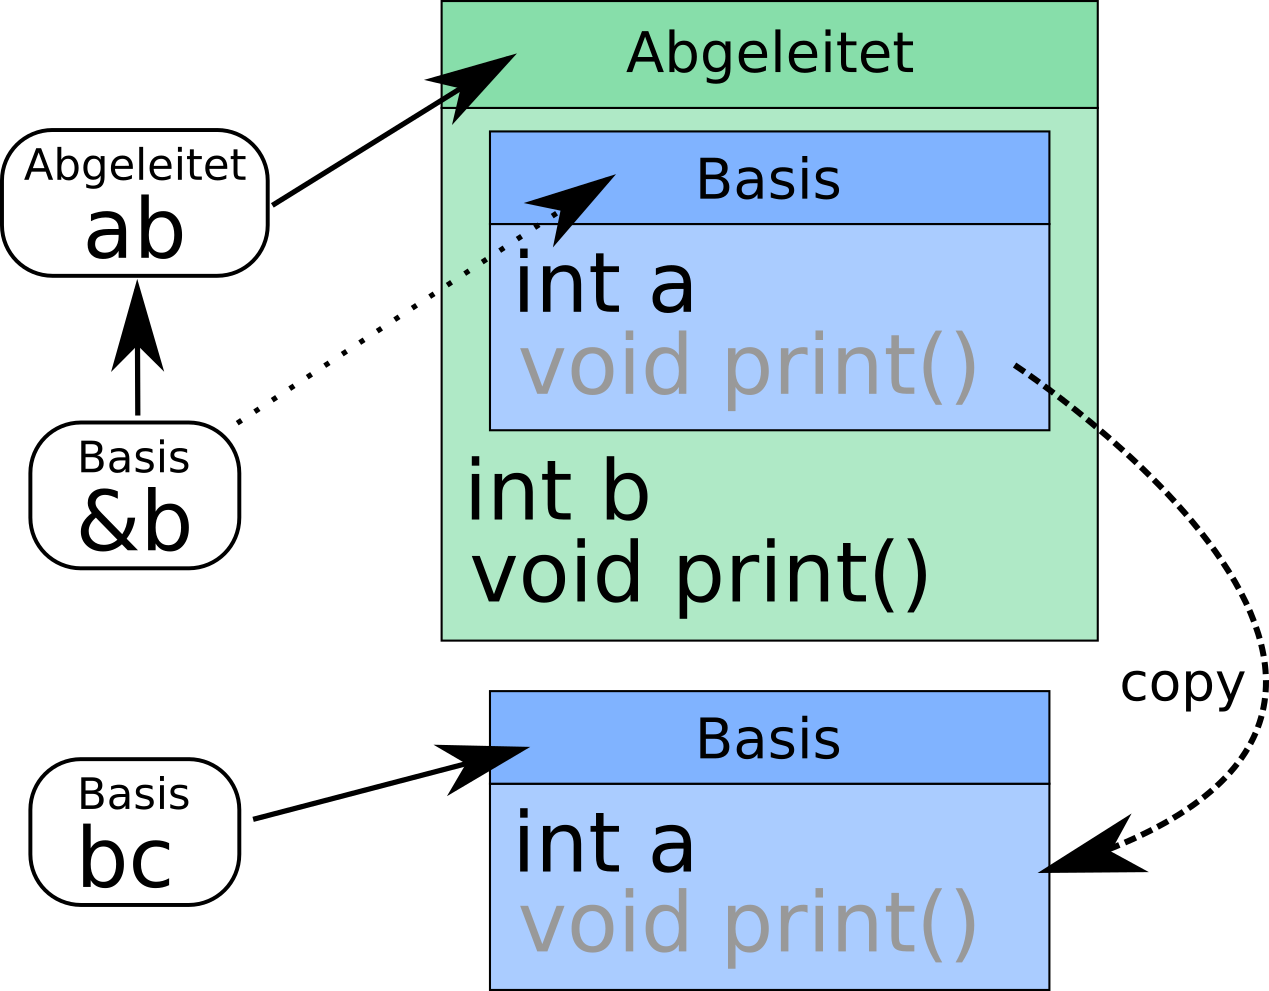
\includegraphics[width=.9\linewidth]{img/slizing_full.png}
\end{center}
\end{frame}
\begin{frame}[label={sec:org665b86c},fragile]{Das Slicing Problem}
 \begin{itemize}
\item Aus Sicht der Referenz {\color{solarizedYellow}\verb!b!} haben wir es nun mit einer Instanz der
Klasse {\color{solarizedYellow}\verb!Basis!} zu tun.

\begin{center}
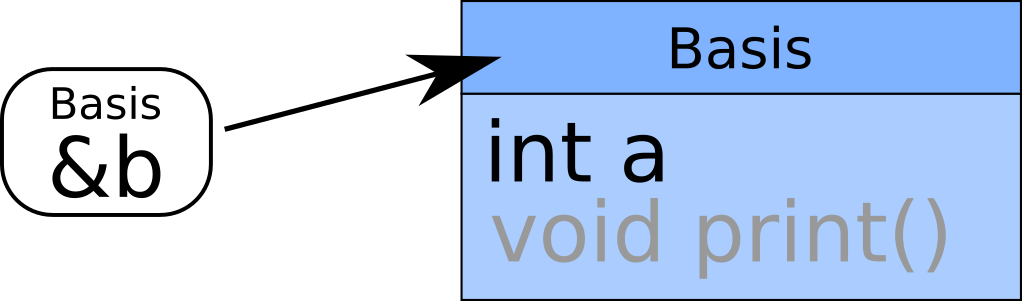
\includegraphics[width=.9\linewidth]{img/slizing_small.png}
\end{center}
\item {\color{solarizedYellow}\verb!b!} hat also "vergessen", dass es auf einen Teil einer
{\color{solarizedYellow}\verb!Abgeleitet!}-Klasse verweist
\item Beim kopieren für die Variable {\color{solarizedYellow}\verb!bc!} wurde nur der Basis-Teil kopiert
\item Man bezeichnet das als Slicing-Problem, weil Teile einer Klasse
tatsächlich, oder scheinbar abgeschnitten werden
\end{itemize}
\end{frame}
\begin{frame}[label={sec:orgb22d80d}]{Der Upcast --- Was passiert}
\begin{center}
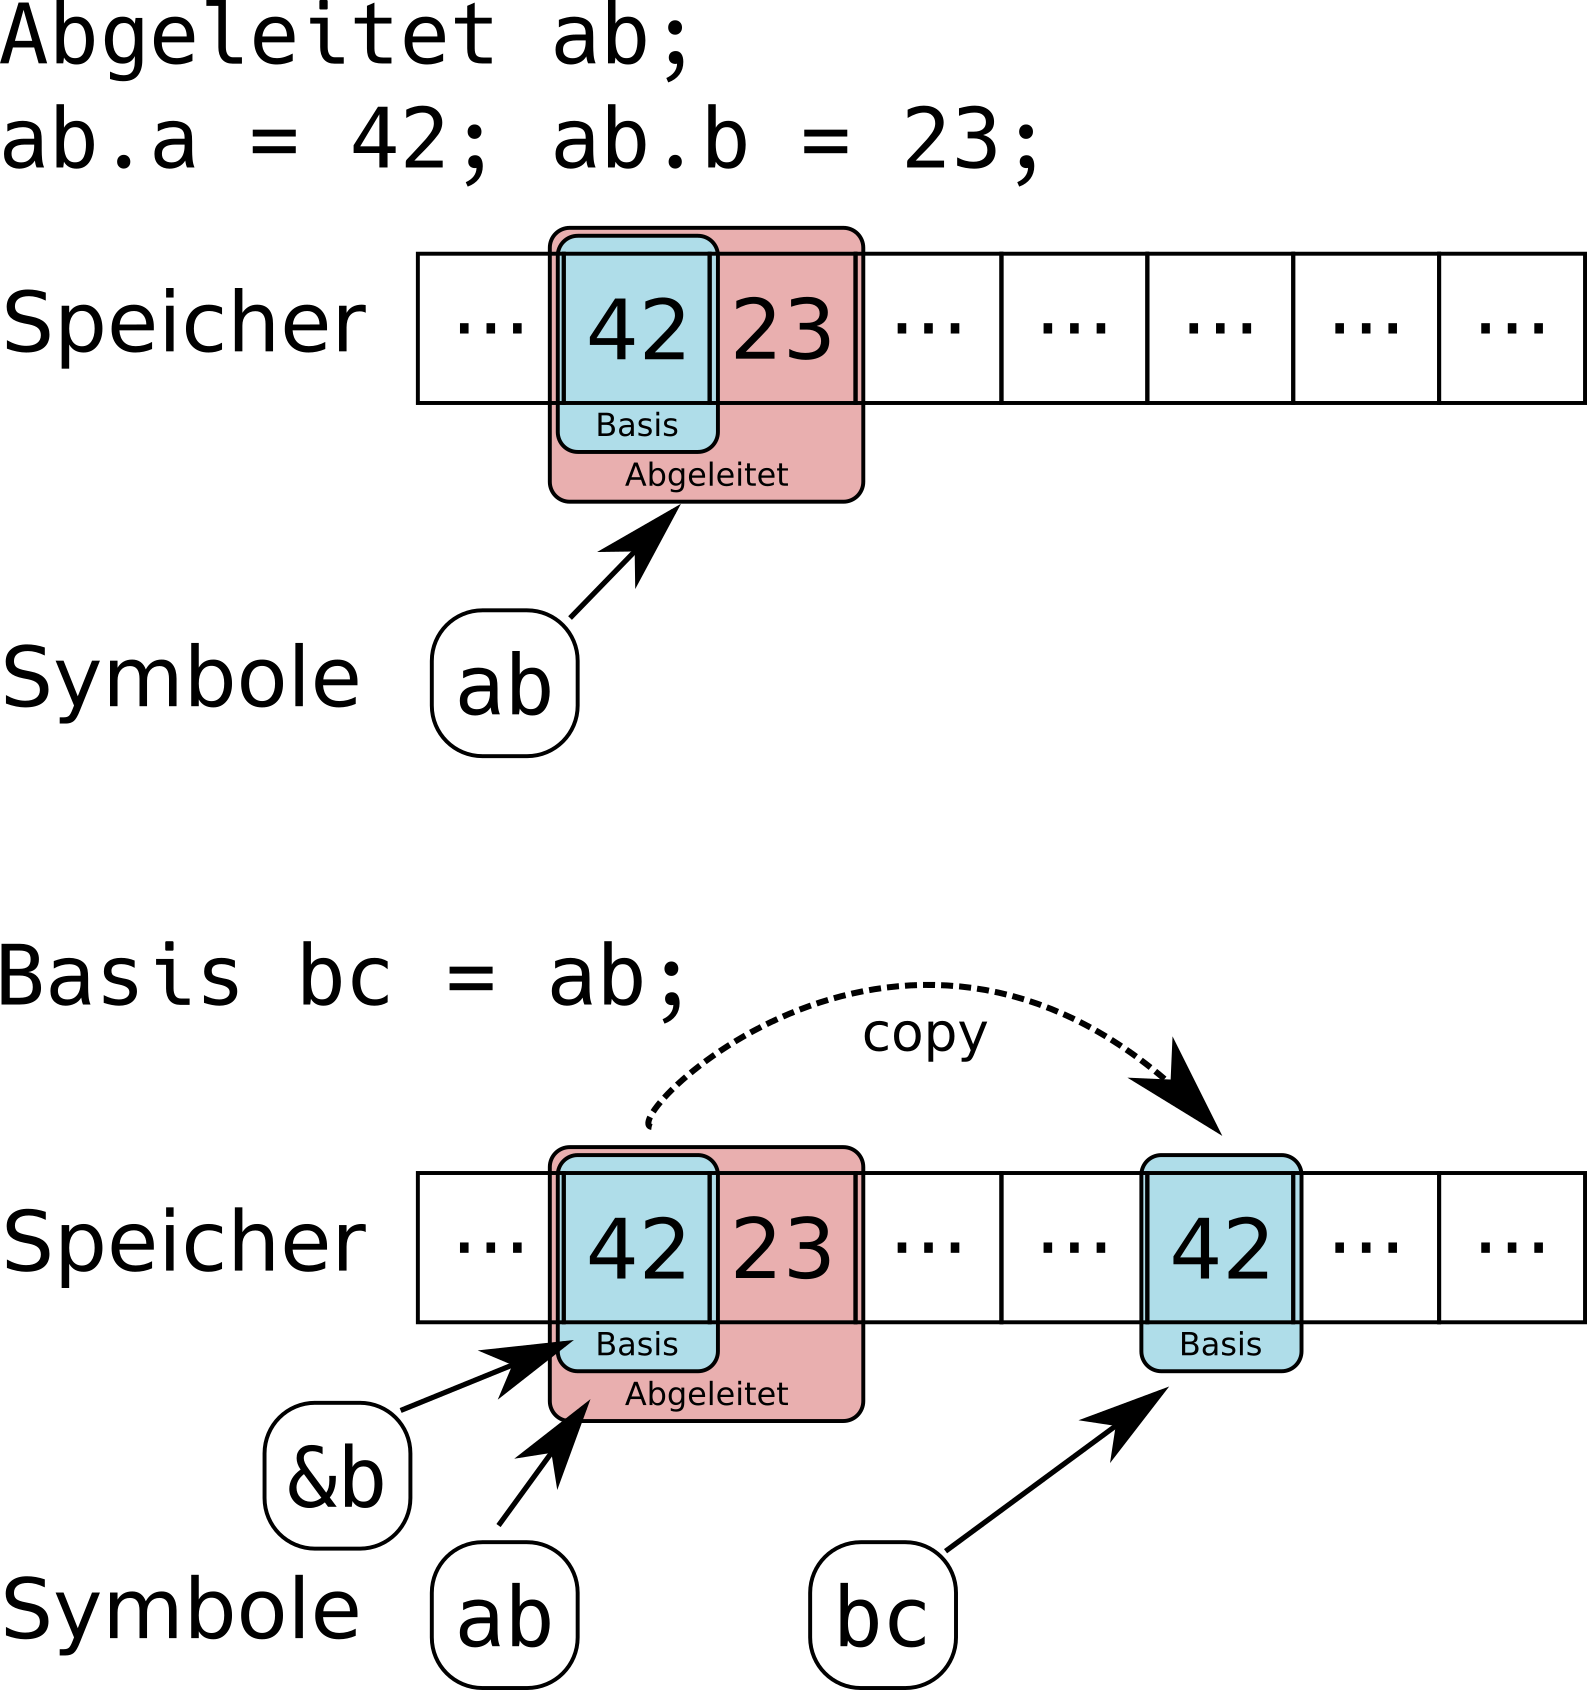
\includegraphics[width=0.65\textwidth]{img/upcast.png}
\end{center}
\end{frame}
\begin{frame}[label={sec:org8f85a01},fragile]{Der Upcast --- Parameter Beispiel}
 \begin{minted}[numberblanklines=false,fontsize=\scriptsize]{c++}
#include <iostream>
using namespace std;

class Basis {
public:
  int a;
  void print() { cout << "Basisklasse mit Nummer " << a << endl; }
};

class Abgeleitet : public Basis {
public:
  int b;
    void print() { cout << "Abgeleitete Klasse mit Nummern " << a
			<< " und " << b << endl; }
};

void callmyprint(Basis &b) { b.print(); }

int main() {
  Abgeleitet ab;
  ab.a = 42; ab.b = 23;
  ab.print(); // Abgeleitete Klasse mit Nummern 42 und 23
  callmyprint(ab); // Basisklasse mit Nummer 42
  // ab wird implizit in Basis konvertiert
}
\end{minted}
\end{frame}
\begin{frame}[label={sec:org293e6b1}]{Effekt eines Upcasts}
\begin{itemize}
\item Wird eine abgeleitete Klasse in den Typ einer Basisklasse
konvertiert, vergisst die Instanz was sie vorher einmal war und
verhält sich dann als wäre es schon immer eine Basisklasse gewesen
\item Dieses Verhalten bezeichnet mal als \alert{slicing} und ist oft nicht was
man will
\item Auf den nächsten Slides werden wir uns das Problem näher ansehen und
mit sogenanntem \alert{Polymorphismus} eine Lösung finden
\end{itemize}
\end{frame}
\section{Polymorphismus}
\label{sec:org63e62ae}
\begin{frame}[label={sec:org3b2370c},fragile]{Ein kleines Beispiel}
 \begin{minted}[numberblanklines=false,fontsize=\scriptsize]{c++}
#include <iostream>
using namespace std;

class Basis {
public: void print() { cout << "Hallo von der Basisklasse" << endl; }
};
class Abgeleitet1 : public Basis {
public: void print() { cout << "Hallo von der abgeleiteten Klasse 1" << endl; }
};
class Abgeleitet2 : public Basis {
public: void print() { cout << "Hallo von der abgeleiteten Klasse 2" << endl; }
};

void print_with_introduction(Basis &a) {
  cout << "Unsere Klasse möchte folgendes sagen: " << endl;
  a.print();
}

int main() {
  Basis b; Abgeleitet1 a1; Abgeleitet2 a2;

  print_with_introduction(b);
  print_with_introduction(a1);
  print_with_introduction(a2);
}
\end{minted}
\end{frame}
\begin{frame}[label={sec:org289cfb0},fragile]{Was ist das Problem?}
 \begin{itemize}
\item Wir hätten gerne, dass sich die Klassen mit ihren tatsächlichen
{\color{solarizedYellow}\verb!print!} Funktionen melden und nicht mit der Standardimplementierung
der Basisklasse
\item Das funktioniert aber auf Grund des Slicing-Problems nicht
\end{itemize}
\begin{block}{Lösung}
Die Lösung ist das Schlüsselwort {\color{solarizedYellow}\verb!virtual!}. Wenn in einer Basisklasse
vor einer Funktion {\color{solarizedYellow}\verb!virtual!} steht, so merkt sich die Klasse welche
Funktion einer abgeleiteten Klasse tatsächlich aufgerufen werden muss.
\end{block}
\begin{block}{Warum ist virtual nicht Standard?}
Der Aufruf einer {\color{solarizedYellow}\verb!virtual!}-Funktion ist langsamer, weil das System
zuerst nachsehen muss welche Funktion tatsächlich aufgerufen werden
muss. Zudem verbraucht eine {\color{solarizedYellow}\verb!virtual!}-Funktion Speicher in jeder
Instanz einer Klasse, weil irgendwo gespeichert werden muss welche
Funktion wirklich aufzurufen ist.
\end{block}
\end{frame}
\begin{frame}[label={sec:org2686708},fragile]{Virtual --- Beispiel}
 \begin{minted}[numberblanklines=false,fontsize=\scriptsize]{c++}
#include <iostream>
using namespace std;

class Basis {
public: virtual void print() { cout << "Hallo von der Basisklasse" << endl; }
};
class Abgeleitet1 : public Basis {
public: void print() { cout << "Hallo von der abgeleiteten Klasse 1" << endl; }
};
class Abgeleitet2 : public Basis {
public: void print() { cout << "Hallo von der abgeleiteten Klasse 2" << endl; }
};

void print_with_introduction(Basis &a) {
  cout << "Unsere Klasse möchte folgendes sagen: " << endl;
  a.print();
}

int main() {
  Basis b; Abgeleitet1 a1; Abgeleitet2 a2;

  print_with_introduction(b);
  print_with_introduction(a1);
  print_with_introduction(a2);
}
\end{minted}
\end{frame}
\begin{frame}[label={sec:org268836a}]{Wann verwendet man Polymorphismus}
\begin{itemize}
\item Man hat eine Basisklasse die ein bestimmtes Verhalten implementiert
\item Davon leitet man mehrere Klassen ab die dieses Verhalten erweitern
\item Man kann jetzt eine Funktion für die Basisklasse schreiben, und als
Parameter alle abgeleiteten Klassen verwenden, oder \ldots{}
\item wir können in einem Vektor oder in einem Array vom Typ der
Basisklasse auch alle abgeleiteten Klassen speichern (als Zeiger
oder Referenz)
\end{itemize}
\end{frame}
\begin{frame}[label={sec:orge98b75b},fragile]{Beispiel --- Vektor mit Zeigern}
 \begin{minted}[numberblanklines=false,fontsize=\scriptsize]{c++}
#include <iostream>
#include <vector>
using namespace std;

class Basis {
public: virtual void print() { cout << "Hallo von der Basisklasse" << endl; }
};
class Abgeleitet : public Basis {
public: void print() { cout << "Hallo von der abgeleiteten Klasse 1" << endl; }
};

int main() {
  vector<Basis *> vec;
  Basis b1, b2;
  Abgeleitet a1, a2;
  vec.push_back(&b1);
  vec.push_back(&b2);
  vec.push_back(&a1);
  vec.push_back(&a2);

  for (auto &e : vec)
    (*e).print();
}
\end{minted}
\end{frame}
\begin{frame}[label={sec:org31c92d5},fragile]{Beispiel --- Vektor mit Referenzen}
 \begin{minted}[numberblanklines=false,fontsize=\scriptsize]{c++}
#include <functional>
#include <iostream>
#include <vector>

using namespace std;

class Basis {
public:
  virtual void print() { cout << "Hallo von der Basisklasse" << endl; }
};
class Abgeleitet : public Basis {
public:
  void print() { cout << "Hallo von der abgeleiteten Klasse 1" << endl; }
};

int main() {
  vector<reference_wrapper<Basis>> vec;
  Basis b1, b2;
  Abgeleitet a1, a2;
  vec.push_back(b1); vec.push_back(b2);
  vec.push_back(a1); vec.push_back(a2);

  for (Basis &e : vec)
    e.print();
}
\end{minted}
\end{frame}
\begin{frame}[label={sec:org9ce2def},fragile]{Übung --- Employee und Manager}
 \footnotesize
\begin{itemize}
\item Implementieren Sie die beiden Klassen {\color{solarizedYellow}\verb!Employee!} und {\color{solarizedYellow}\verb!Manager!}
\item {\color{solarizedYellow}\verb!Employee!} ist die Basisklasse, {\color{solarizedYellow}\verb!Manager!} ist die abgeleitete
Klasse. Ein Manager ist also auch ein Angestellter
\item {\color{solarizedYellow}\verb!Employee!} hat eine Variable {\color{solarizedYellow}\verb!salary!} die speichert wie viel der
jeweilige Mitarbeiten verdient
\item {\color{solarizedYellow}\verb!Employee!} hat eine Funktion {\color{solarizedYellow}\verb!raise!} mit der man einem Mitarbeiter
eine Gehaltserhöhung geben kann. Damit der unsere Mitarbeiter nicht
zu viel verdienen, wird der maximale Gehalt auf {\color{solarizedYellow}\verb!3500!} beschränkt
\item {\color{solarizedYellow}\verb!Employee!} hat auch eine Funktion {\color{solarizedYellow}\verb!print!} die ausgibt: {\color{solarizedYellow}\verb!Der
  Mitarbeiter hat einen Gehalt von ...!}
\item Im {\color{solarizedYellow}\verb!Manager!} wird die Funktion {\color{solarizedYellow}\verb!raise!} überladen und das Gehalt ist
nicht beschränkt
\end{itemize}
\begin{block}{Verwendung}
\begin{itemize}
\item Erzeugen Sie einen Vektor und füllen Sie ihn mit einigen {\color{solarizedYellow}\verb!Employee!}
sowie {\color{solarizedYellow}\verb!Manager!} Instanzen (entweder mit Zeigern oder Referenzen)
\item Iterieren Sie über den Vektor und rufen {\color{solarizedYellow}\verb!raise!} sowie {\color{solarizedYellow}\verb!print!} auf
und beobachten Sie das Verhalten
\end{itemize}
\end{block}
\end{frame}
\begin{frame}[label={sec:org22aa3cb}]{Hinweis}
\begin{itemize}
\item \alert{Polymorphismus} ist ein weiterführendes Thema der
Objektorientierten Programmierung und uns fehlen einige Grundlagen
um das Konzept wirklich gut nützen zu können (z.B. dynamische
Speicherverwaltung)
\item Es geht in erster Linie darum, \alert{dass sie das Konzept gehört haben}
und sich zumindest ungefähr vorstellen können um was es geht
\item Sie müssen Polymorphismus im Abschlussprojekt nicht verwenden.
\end{itemize}
\end{frame}
\end{document}
